\documentclass[a4paper, 12pt]{report}

% Packages
\usepackage{alltt, fancyvrb, url}
\usepackage{graphicx}
\usepackage[margin=2cm]{geometry}
\usepackage[utf8]{inputenc}
\usepackage{float}
\usepackage{hyperref}
\usepackage{multicol}
\usepackage{xurl}
\usepackage{lipsum}
\usepackage[htt]{hyphenat}
\usepackage{tabularx}
\usepackage{array}
\usepackage{color}
\usepackage{colortbl}
\usepackage[table]{xcolor}
\usepackage[font={small,it}]{caption}

% Language Package
\usepackage[italian]{babel}
\usepackage[italian]{cleveref}
\usepackage[toc,page]{appendix}

% Definition of environments and colors
\definecolor{seaGreen}{cmyk}{0.19, 0, 0.25, 0.09}

\newenvironment{sloppypar*}{\sloppy\ignorespaces}{\par}

\newenvironment{changemargin}[2]{%
  \begin{list}{}{%
    \setlength{\topsep}{0pt}%
    \setlength{\leftmargin}{#1}%
    \setlength{\rightmargin}{#2}%
    \setlength{\listparindent}{\parindent}%
    \setlength{\itemindent}{\parindent}%
    \setlength{\parsep}{\parskip}%
  }%
  \item[]}{\end{list}}

\newenvironment{packed_enum}{
\begin{enumerate}
        \setlength{\itemsep}{1pt}
        \setlength{\parskip}{0pt}
        \setlength{\parsep}{0pt}
}{\end{enumerate}}

% Initialization
\title{Relazione Progetto Basi di Dati 2022}
\author{Michele Montesi \\
        Matricola: 0000974934 \\
        E-Mail: michele.montesi3@studio.unibo.it}

\date{\today}

% Begin
\begin{document}
    
\maketitle
\tableofcontents

\chapter{Analisi Dei Requisiti}
Si vuole realizzare un database a supporto dell'automatizzazione della gestione di una
comunità la quale gestisce diverse residenze per pazienti psichiatrici.
La base di dati dovrà immagazzinare informazioni relative agli operatori, ai pazienti e
alle varie residenze.

\section{Intervista}
Un primo testo ottenuto dall'intervista è il seguente:

\begin{changemargin}{0.5cm}{0.5cm}
        \noindent
        Si vuole tenere traccia di \textbf{pazienti} e \textbf{dipendenti} memorizzandone le informazioni personali
        quali codice fiscale, nome, cognome, compleanno e sesso.
        Differenziando le due entità si memorizzeranno, inoltre, le informazioni legate alla propria posizione.
        Questi due soggetti possono essere registrati nel sistema solo accettando alcune clausole o
        disponendo di eventuali requisiti.\\
        I \textbf{dipendenti} possono acquisire degli \textbf{attestati} che gli conferiscono crediti ECM e possono firmare
        \textbf{contratti} (prima di firmare un secondo contratto con lo stesso nome, il primo deve essere concluso).
        Di entrambi verrà mantenuto uno storico.\\
        I \textbf{turni} dei dipendenti sono determinati dal codice fiscale del dipendente, il giorno della settimana, 
        l'ora d'inizio, l'ora di fine e l'unità operativa in cui si svolgeranno.\\
        I \textbf{pazienti} sono identificati da una \textbf{cartella clinica} la quale contiene informazioni riguardanti
        l'anamnesi, la diagnosi e il progetto riabilitativo del paziente. A ognuno di questi verrà assegnata una 
        \textbf{terapia} la quale dovrà essere seguita assumendo farmaci (somministrati da dipendenti) e della quale
        verrà mantenuto uno storico.\\
        I \textbf{farmaci} sono caratterizzati dal loro codice, il nome, la casa farmaceutica, le date d'acquisto e
        di scadenza e la quantità.\\
        Sono presenti \textbf{unità operative} (le quali possono essere \texttt{gruppi appartamento} o \texttt{residenze
        sanitarie psichiatriche}) adibite all' \textbf{ospitazione} di più pazienti (la quale dovrà essere registrata
        con data d'inizio e opzionalmente con una data di fine) della quale verrà mantenuto uno storico.
        Queste sono caratterizzate dalla loro ubicazione, i posti letto e il numero dei pazienti.
        Per poter essere operative devono ricevere l'\texttt{autorizzazione al funzionamento} e l'\texttt{accreditamento}.
        Ogni unità operativa avrà una lista di \textbf{beni strumentali}, i quali possono essere automezzi o attrezzature.
\end{changemargin}

\section{Estrazione dei concetti principali}\label{sec:estrazione-dei-concetti-principali}
\begin{tabularx}{\textwidth}{lXc}
        \rowcolor{seaGreen}
        \textbf{Termine} & \textbf{Breve descrizione} & \textbf{Eventuali sinonimi} \\
        Dipendente & Colui che è assunto dalla società e lavora in una o più strutture a seconda dei turni e
        somministra farmaci ai pazienti.\ Può essere socio.\ & Lavoratore \\
        \hline
        Contratto & Oggetto contenente le ore lavorative mensili del dipendente a cui viene sottoscritto.\ & Contratto Lavorativo \\
        \hline
        Attestato & Oggetto che conferisce, al dipendente che ne consegue il completamento, crediti EMC (crediti formativi).\ & Formazione \\
        \hline
        Paziente & Colui che riceve le cure attraverso la somministrazione di farmaci, seguendo una terapia, ed è ospitato
        all'interno di una unità operativa.\ & Cliente \\
        \hline
        Cartella clinica & Documentazione del paziente contenente anamnesi, diagnosi e progetto riabilitativo.\ & Cartella \\
        \hline
        Terapia & Oggetto che riporta i farmaci da assumere durante un periodo di tempo.\ & Cura \\
        \hline
        Farmaco & Medicinale adibito all'assunzione da parte di pazienti a cui è stato assegnato.\ & Medicinale \\
        \hline
        Unità operativa & Residenza o appartamento i cui i pazienti risiedono e ricevono le cure da parte del personale.\ & Residenza, Unità \\
        \hline
        Bene strumentale & Strumento o veicolo aziendale necessario o utile a semplificare il lavoro o la permanenza nell'unità operativa.\ & Strumentazione, Veicolo
\end{tabularx}
\\\\\\
A seguito della lettura e comprensione dei requisiti, si procede redigendo un testo che ne 
riassuma tutti i concetti e in particolare ne estragga quelli principali eliminando le ambiguità 
sopra rilevate:

\begin{changemargin}{0.5cm}{0.5cm}
        \noindent
        Per ogni \textbf{dipendente} vengono memorizzati Codice Fiscale, Nome, Cognome, Compleanno, Residenza, Sesso, Titolo di Studio,
        l'Idoneità alla mansione, se è Socio o meno e i Crediti ECM. Ogni dipendente dispone, inoltre, di un codice univoco fornitogli
        al momento del suo inserimento nel DB. 
        Ogni dipendente può acquisire degli \textbf{attestati} che gli conferiscono crediti ECM e possono firmare
        \textbf{contratti} (prima di firmare un secondo contratto con lo stesso nome, il primo deve essere concluso).
        Di entrambi verrà mantenuto uno storico.\\
        I \textbf{turni} dei dipendenti sono determinati dal codice fiscale del dipendente, il giorno della settimana, 
        l'ora d'inizio, l'ora di fine e l'unità operativa in cui si svolgeranno. Un turno di uno stesso dipendente nello stesso
        giorno della settimana non potrà essere definito se si interseca ad un altro.\\
        Per ogni \textbf{paziente} vengono memorizzati Codice Fiscale, Nome, Cognome, Compleanno, Residenza, Sesso.
        Al momento della registrazione dovrà firmare la documentazione alla privacy, il consenso al trattamento e l'accettazione
        del regolamento. Ognuno possiede una \textbf{cartella clinica} la quale contiene informazioni riguardanti
        l'anamnesi, la diagnosi e il progetto riabilitativo. A ognuno di questi verrà assegnata una 
        \textbf{terapia} la quale dovrà essere seguita assumendo farmaci (somministrati da dipendenti) e della quale
        verrà mantenuto uno storico.\\
        Ogni \textbf{farmaco} è caratterizzato dal loro codice, il nome, la casa farmaceutica, le date d'acquisto e
        di scadenza e la quantità.\\
        Ogni \textbf{unità operativa} può essere \texttt{gruppo appartamento} o \texttt{residenza sanitaria psichiatrica}.
        Ognuna di queste è adibita all' \textbf{ospitazione} di più pazienti (la quale dovrà essere registrata
        con data d'inizio e opzionalmente con una data di fine) della quale verrà mantenuto uno storico.
        Ognuna è caratterizzate dall'ubicazione, i posti letto e il numero dei pazienti.
        Per poter essere operative devono ricevere l'\texttt{autorizzazione al funzionamento} e l'\texttt{accreditamento}.
        Ogni unità operativa avrà una lista di \textbf{beni strumentali}, i quali possono essere automezzi o attrezzature.
        \newline
\end{changemargin}
Segue un elenco delle principali operazioni richieste:
\begin{packed_enum}
        \item Registrare un nuovo dipendente
        \item Registrare un turno
        \item Registrare un nuovo paziente
        \item Registrare un farmaco
        \item Registrare una nuova unità operativa
        \item Registrare un contratto
        \item Registrare un attestato
        \item Assegnare un contratto ad un dipendente
        \item Assegnare un attestato ad un dipendente
        \item Far assumere un farmaco ad un paziente
        \item Visualizzare tutti i dipendenti
        \item Visualizzare tutti i pazienti
        \item Visualizzare tutti i turni
\end{packed_enum}

\chapter{Progettazione Concettuale}

\section{Schema scheletro}

% Dipendente e Paziente
\noindent
Le entità di \textbf{dipendente} e \textbf{paziente} sono la generalizzazione di una entità \textbf{persona}, identificata
tramite il codice fiscale. Ogni paziente possiede una terapia la quale gli viene somministrata da un dipendente.
Quando questa viene somministrata, in base alla quantità di farmaci utilizzati, il contatore del farmaco in questione verrà
diminuito di tale dato.

\begin{figure}[H]
        \centering
        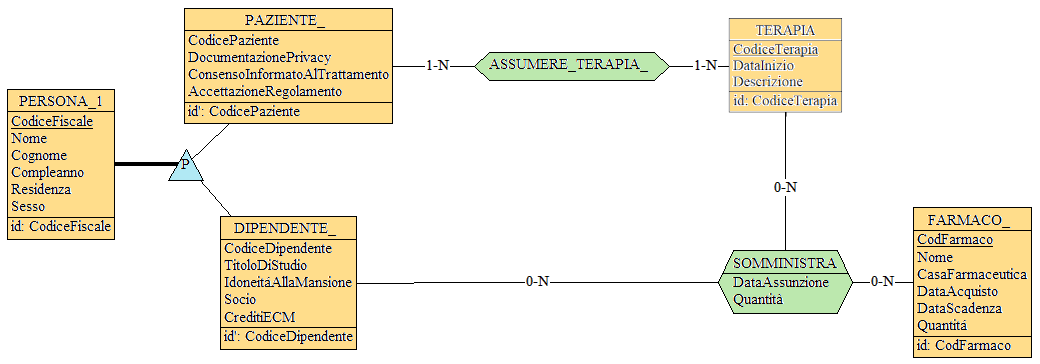
\includegraphics[height=5cm]{img/dipendentePazienteERPostReif.png}
        \caption{Schema E/R con le principali entità per modellazione della somministrazione di farmaci}
\end{figure}

\noindent
Dall'analisi del dominio si evince come serva tenere uno storico di tutti i farmaci somministrati
da un dipendente ad un paziente. Perciò si reifica l'associazione tra \textbf{dipendente} e \textbf{terapia} generando
una nuova entità \textbf{farmaco\_terapia} che tiene traccia della quantità del \textbf{farmaco} somministrato, la data, 
il somministratore e la terapia. Questa entità è definita dal suo \textit{codice univoco incrementale}, il \textit{codice della terapia} ed 
il \textit{codice del dipendente}.

\begin{figure}[H]
        \centering
        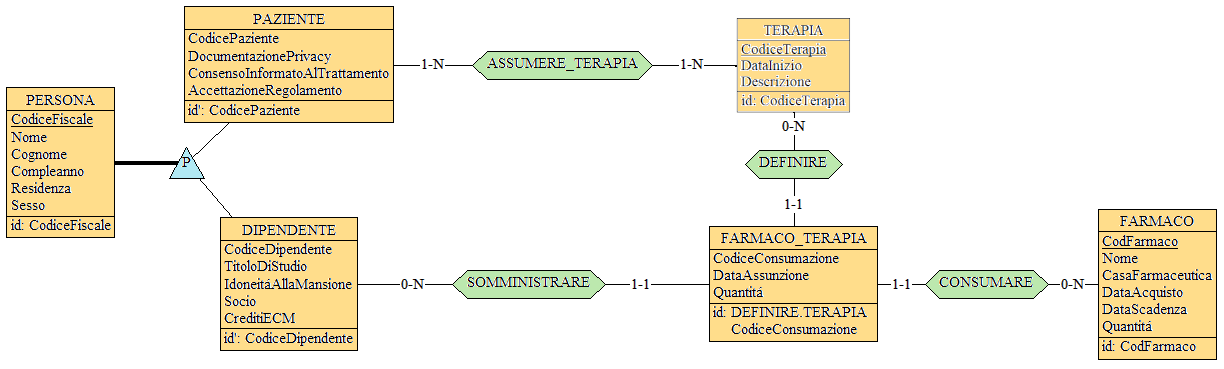
\includegraphics[height=5cm]{img/dipendentePazienteERPreReif.png}
        \caption{Schema E/R con le principali entità per modellazione della somministrazione di farmaci e del suo storico}
\end{figure}

% Dipendente
\noindent
Un dipendente durante la sua carriera può acquisire \textbf{contratti} e \textbf{attestati}, i quali verranno registrati con le proprie date
di acquisizione ed eventualmente di fine validità.

\begin{figure}[H]
        \centering
        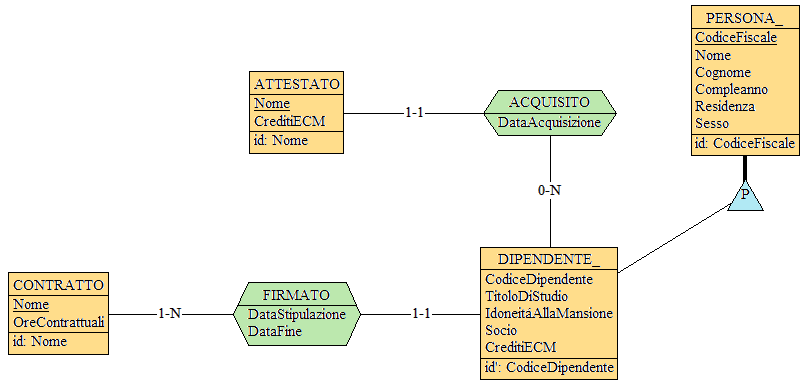
\includegraphics[height=6cm]{img/dipendenteContrattiPreReif.png}
        \caption{Schema E/R rappresentante il sistema di contratti e attestati per i dipendenti}
\end{figure}

\noindent
Poiché ogni dipendente può firmare più di un contratto e può acquisire più di un attestato non è sufficiente un'associazione.
Viene, quindi, eseguita la reificazione delle due associazioni interessate creando due nuove entità, grazie alle quali sarà possibile
mantenere uno storico degli \textbf{attestati acquisiti} e dei \textbf{contratti stipulati}, potendone registrare più di uno per dipendente.

\begin{figure}[H]
        \centering
        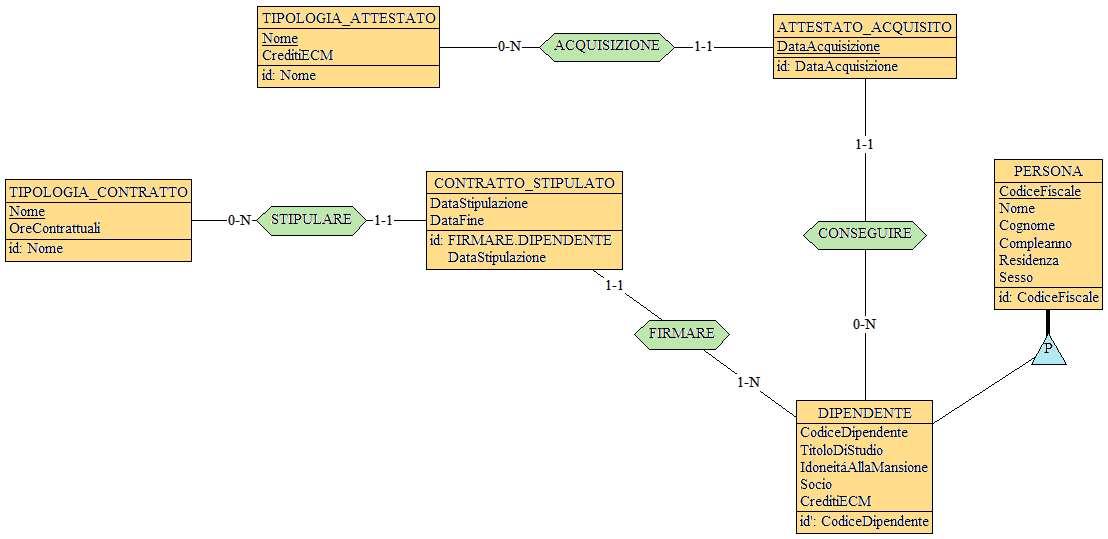
\includegraphics[height=8cm]{img/dipendenteContrattiPostReif.png}
        \caption{Schema E/R rappresentante il sistema di contratti e attestati per i dipendenti e la loro storicizzazione}
\end{figure}

\noindent
Ogni paziente possiede una tabella rappresentante i propri turni dal lunedì alla domenica. Ogni turno è identificato dall'unità operativa
in cui verrà svolto, dal giorno della settimana, l'ora d'inizio e dal dipendente da cui verrà svolto.
\begin{figure}[H]
        \centering
        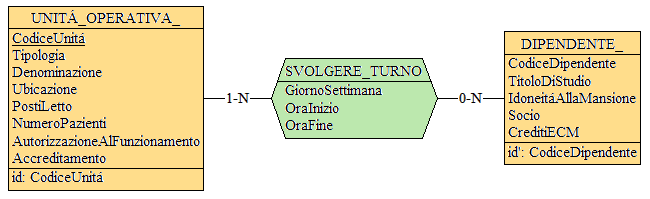
\includegraphics[height=4cm]{img/dipendenteTurniPreReif.png}
        \caption{Schema E/R rappresentante il sistema di turni per ogni paziente}
\end{figure}

\noindent
Poiché ogni dipendente può svolgere più di un turno è stato necessario operare una reificazione dell'associazione tra dipendente
e unità operativa. In questo modo si potrà tenere più di un turno per ogni dipendente, a patto che questi non siano in sovrapposizione.

\begin{figure}[H]
        \centering
        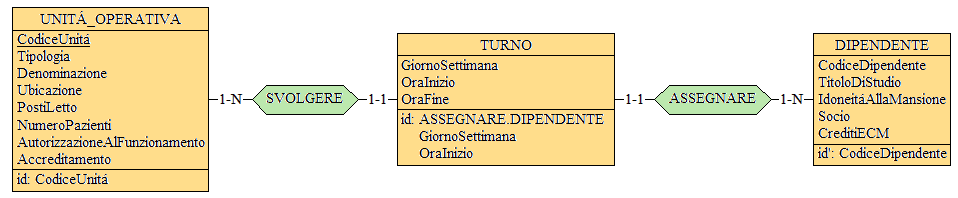
\includegraphics[height=3.5cm]{img/dipendenteTurniPostReif.png}
        \caption{Schema E/R rappresentante il sistema di turni per ogni paziente e la tabella dei turni}
\end{figure}

% Paziente
\noindent
Un paziente può essere ospitato in un'\textbf{unità operativa}. Nelle informazioni che vanno registrate al momento dell'inserimento è presente
la data d'inizio permanenza e opzionalmente la data di fine.

\begin{figure}[H]
        \centering
        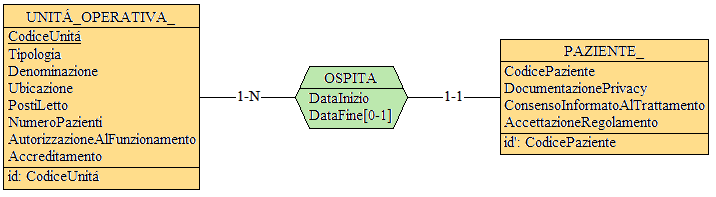
\includegraphics[height=4cm]{img/pazienteOspitazionePreReif.png}
        \caption{Schema E/R rappresentante il sistema di ospitazione dei pazienti nelle unità operative}
\end{figure}

\noindent
Poiché ogni paziente può essere ospitato in più unità operative in diversi periodi di tempo, è necessario operare la reificazione
dell'associazione tra paziente e unità operativa. Così facendo sarà possibile mantenere uno storico di tutte le \textbf{ospitazioni},
potendone inserire più di una per paziente.

\begin{figure}[H]
        \centering
        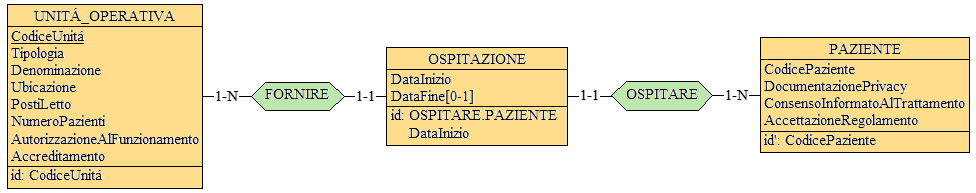
\includegraphics[height=3cm]{img/pazienteOspitazionePostReif.png}
        \caption{Schema E/R rappresentante il sistema di ospitazione dei pazienti nelle unità operative e la loro storicizzazione}
\end{figure}

\noindent
Ogni paziente è identificato da una, ed una soltanto, \textbf{cartella clinica}, per cui è stata sufficiente e necessaria un'associazione
1-1 tra i due soggetti interessati. In ogni cartella clinica sono presenti informazioni personali per ogni paziente quali l'\textit{anamnesi},
la \textit{diagnosi} e il proprio \textit{progetto riabilitativo}. 

\begin{figure}[H]
        \centering
        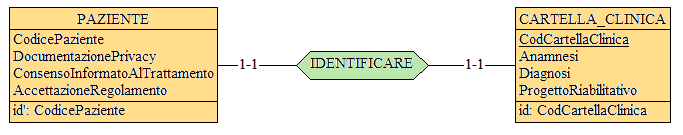
\includegraphics[height=3cm]{img/pazienteCartella.png}
        \caption{Schema E/R rappresentante la relazione tra paziente e cartella clinica}
\end{figure}

% Unità Operativa
\noindent
Ogni unità operativa possiede diversi \textbf{beni strumentali} i quali possono essere \textbf{attrezzature} oppure \textbf{automezzi}.
Ogni bene strumentale appartiene ad una, ed una soltanto, unità operativa. Le entità \texttt{attrezzatura} e \texttt{automezzi} sono una generalizzazione
dell'entità \texttt{beni\_strumentali}. Nel caso di \texttt{attrezzatura} verrà registrato, oltre alle informazioni del supertipo, il nome dell'attrezzo.
Nel caso di \texttt{automezzi} verrà registrata, invece, la targa, la tipologia di veicolo e la scadenza della sua assicurazione.

\begin{figure}[H]
        \centering
        \includegraphics[height=10cm]{img/unitàOperativaBeni.png}
        \caption{Schema E/R rappresentante la relazione tra unità operativa e beni strumentali}
\end{figure}

\section{Schema finale}

\begin{figure}[H]
        \centering
        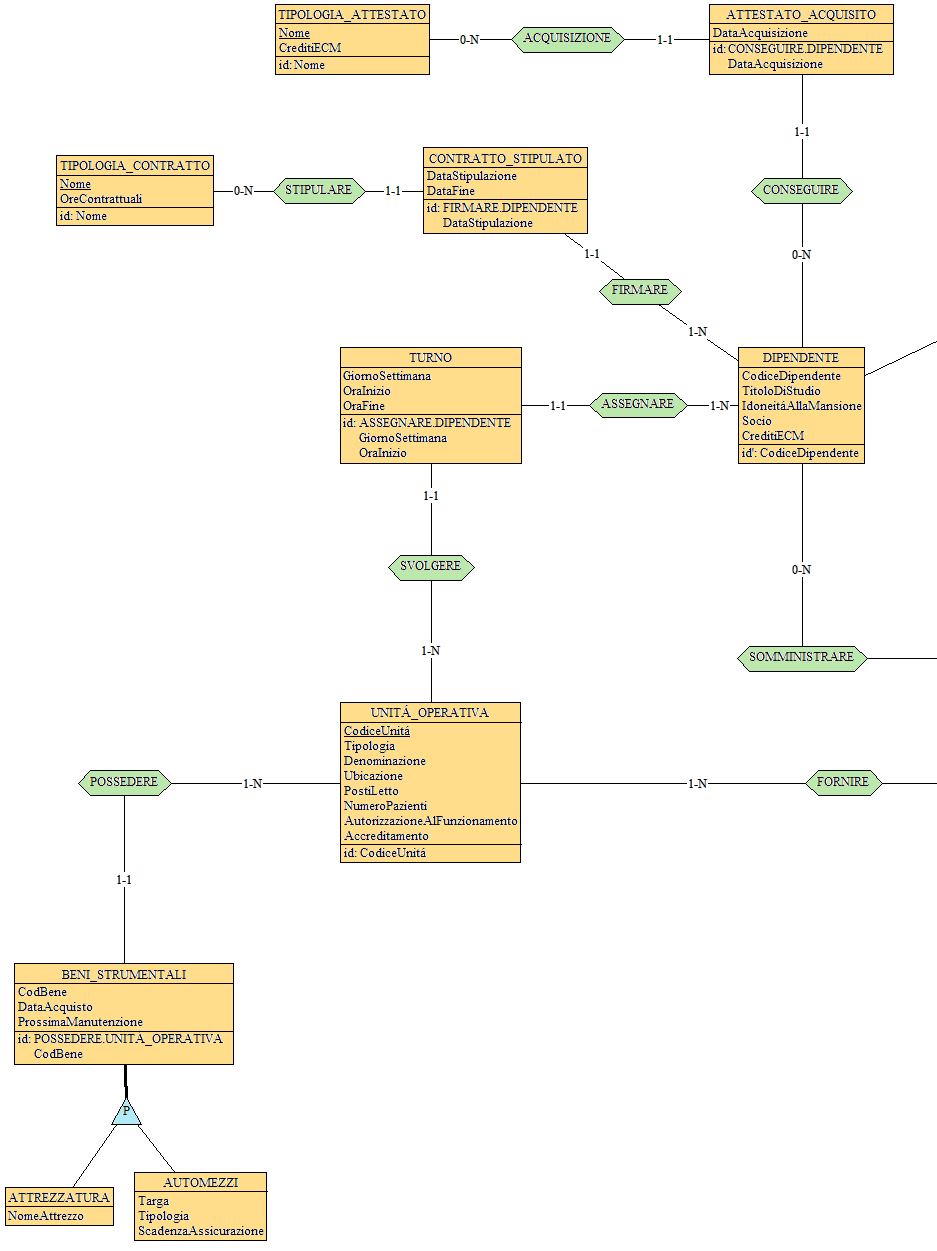
\includegraphics[width=1.0\textwidth]{img/ERFinaleSX.png}
\end{figure}

\begin{figure}[H]
        \centering
        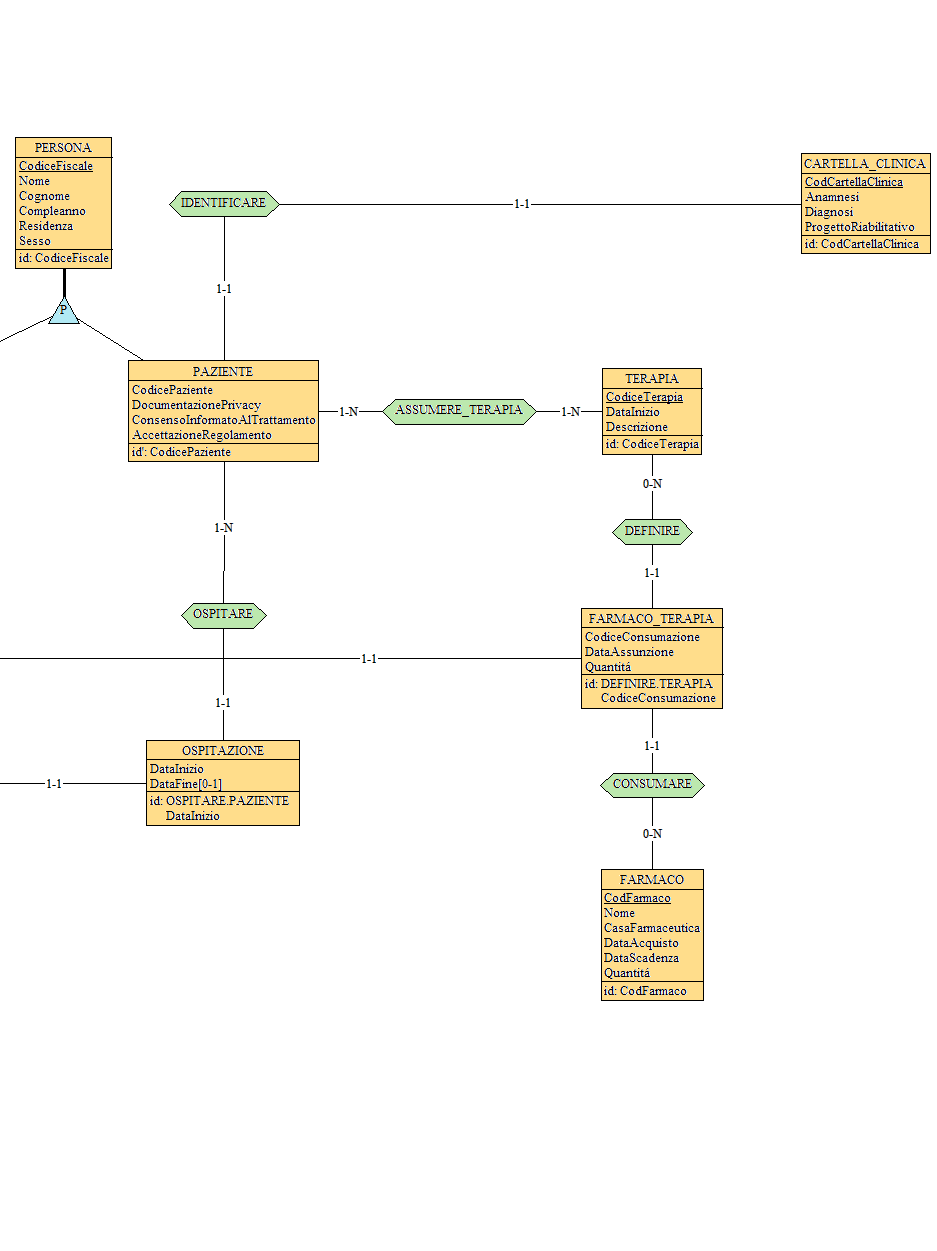
\includegraphics[width=1.0\textwidth]{img/ERFinaleDX.png}
\end{figure}

\chapter{Progettazione Logica}

\section{Stima del volume dei dati}

\begin{changemargin}{-1cm}{-1cm}
        \begin{multicols}{2}
                \renewcommand{\arraystretch}{1.2}
                \begin{tabularx}{8.5cm}{lXc}
                        \rowcolor{seaGreen}
                        \textbf{Concetto} & \textbf{Costrutto} & \textbf{Volume} \\
                        Dipendente & E & 500 \\
                        \hline
                        Assegnare & R & 10000 \\
                        \hline
                        Turno & E & 10000 \\
                        \hline
                        Svolgere & R & 10000 \\
                        \hline
                        Unità Operativa & E & 50 \\
                        \hline
                        \vspace{\baselineskip} \\
                        \hline
                        Tipologia Attestato & E & 50 \\
                        \hline
                        Acquisizione & R & 2500 \\
                        \hline
                        Attestato Acquisito & E & 2500 \\
                        \hline
                        Conseguire & R & 2500 \\
                        \hline
                        \vspace{\baselineskip} \\
                        \hline
                        Tipologia Contratto & E & 20 \\
                        \hline
                        Stipulare & R & 1000 \\
                        \hline
                        Contratto Stipulato & E & 1000 \\
                        \hline
                        Firmare & R & 1000 \\
                        \hline
                        \vspace{\baselineskip} \\
                        \hline
                        Paziente & E & 2000 \\
                        \hline
                        Identificare & R & 2000 \\
                        \hline
                        Cartella Clinica & E & 2000 \\
                        \hline
                        \vspace{\baselineskip} \\
                        \hline
                        Terapia & E & 1500 \\
                        \hline
                        Assumere Terapia & R & 2000 \\
                        \hline
                        Definire & R & 1000 \\
                        \hline
                        Farmaco Terapia & E & 10000 \\
                        \hline
                        Somministrare & R & 10000 \\
                        \hline
                        Consumare & R & 10000 \\
                        \hline
                        Farmaco & E & 1000 \\
                        \hline
                \end{tabularx}

                \begin{tabularx}{8.5cm}{lXc}
                        \rowcolor{seaGreen}
                        \textbf{Concetto} & \textbf{Costrutto} & \textbf{Volume} \\
                        Ospitare & R & 8000 \\
                        \hline
                        Ospitazione & E & 8000 \\
                        \hline
                        Fornire & R & 8000 \\
                        \hline
                        Possedere & R & 5000 \\
                        \hline
                        Beni Strumentali & E & 5000 \\
                        \hline
                \end{tabularx}
        \end{multicols}
\end{changemargin}

\section{Descrizione delle operazioni principali e stima della loro frequenza}

\renewcommand{\arraystretch}{1.2}
\begin{tabularx}{\textwidth}{cXl}
        \rowcolor{seaGreen}
        \textbf{Codice} & \textbf{Operazione} & \textbf{Frequenza} \\
        1 & Registrare un nuovo dipendente & 10 all'anno \\
        \hline
        2 & Registrare un nuovo paziente & 5 al mese \\
        \hline
        3 & Registrare la somministrazione di un farmaco & 2000 al giorno \\
        \hline
        4 & Compilare una nuova cartella clinica & 5 al mese \\
        \hline
        5 & Creare una terapia & 1 al mese \\
        \hline
        6 & Assegnare una terapia già esistente ad un paziente & 5 al mese \\
        \hline
        7 & Aggiornare la terapia di un paziente & 20 all'anno \\
        \hline
        8 & Visualizzare tutti i pazienti con inizio ospitazione in un dato anno & 20 al mese \\
        \hline
        9 & Registrare l'acquisto di beni strumentali & 10 al mese \\
        \hline
        10 & Registrare l'acquisto di farmaci & 15 al mese \\
        \hline
        11 & Visualizzare tutti i pazienti con una data terapia & 10 al giorno \\
        \hline
        12 & Registrare la stipulazione di un contratto già esistente & 10 all'anno \\
        \hline
        13 & Visualizzare tutti i dipendenti con un contratto specifico & 10 al mese\\
        \hline
        14 & Visualizzare tutti i dipendenti di turno in un giorno della settimana & 1 ogni 2 anni \\
        \hline
        15 & Registrare un nuovo turno & 1 al mese \\
        \hline
        16 & Aggiornare un turno già esistente & 10 al mese \\
        \hline
\end{tabularx}

\section{Schemi di navigazione e tabelle degli accessi}

\section{Raffinamento dello schema}

\section{Analisi delle ridondanze}

\section{Traduzione di entità e associazioni in relazioni}

\section{Schema relazionale finale}

\section{Traduzione delle operazioni in query SQL}

\chapter{Progettazione dell’applicazione}

\section{Descrizione dell’architettura dell’applicazione realizzata}

\end{document}